\documentclass[12pt]{article}
\usepackage[a4paper, left=2cm, right=2cm, top=2cm, bottom=2cm]{geometry}
\usepackage[brazil]{babel}
\usepackage{amsmath}
\usepackage{minted}
\usepackage{caption}
\usepackage{subcaption}
\usepackage{graphicx}

\title{Algoritmos e Programação II\\
\large II Lista de Execícios: Array}
\author{Prof. Evandro C. R. Rosa\\UNIVALI}
\date{}

\begin{document}
\maketitle

\noindent Nome Completo: \underline{\hspace{8cm}} Código de Pessoa: \underline{\hspace{2.4cm}}

\begin{enumerate}
      \item Responda sucintamente:
            \begin{enumerate}
                  \item Observe a seguinte definição de array: \texttt{int valores[10];}
                        \begin{enumerate}
                              \item Quantos elementos o array possui?
                              \item Qual é o índice do primeiro elemento no array?
                              \item Qual é o índice do último elemento no array?
                              \item Supondo que um \texttt{int} utilize quatro bytes de memória, quanta memória o array utiliza?
                        \end{enumerate}
                  \item Por que uma função que recebe um array como argumento e o processa também deve aceitar um argumento especificando o tamanho do array?
                  \item Considere a seguinte definição de array: \texttt{int valores[5] = \{ 4, 7, 6, 8, 2 \};} O que cada uma das seguintes instruções exibe?
                        \begin{enumerate}
                              \item \texttt{std::cout << valores[4] << std::endl;}
                              \item \texttt{std::cout << (valores[2] + valores[3]) << std::endl;}
                              \item \texttt{std::cout << ++valores[1] << std::endl;}
                        \end{enumerate}
                  \item Como você define um array sem fornecer um tamanho na declaração?
                  \item Observe a seguinte definição de array: \texttt{int numeros[5] = \{ 1, 2, 3 \};}
                        \begin{enumerate}
                              \item Qual valor está armazenado em \texttt{numeros[2]}?
                              \item Qual valor está armazenado em \texttt{numeros[4]}?
                        \end{enumerate}
                  \item Um array é passado para uma função por valor ou por referência?
                  \item Quando você passa o nome de um array como argumento para uma função, o que é realmente passado?
                  \item Como você estabelece uma relação paralela entre dois ou mais arrays?
                  \item Observe a seguinte definição de array: \texttt{double vendas[8][10];}
                        \begin{enumerate}
                              \item Quantas linhas o array possui?
                              \item Quantas colunas o array possui?
                              \item Quantos elementos o array possui?
                              \item Escreva uma instrução que armazena um número na última coluna da última linha do array.
                        \end{enumerate}
                  \item Ao escrever uma função que aceita um array bidimensional como argumento, qual tamanho deve ser especificado no parâmetro para o array?
            \end{enumerate}

      \item Os códigos abaixo possuem um ou mais erros. Indique quais são:
            \begin{enumerate}
                  \item \begin{minted}{cpp}
      int tamanho;
      double valores[tamanho];
                  \end{minted}
                  \item \begin{minted}{cpp}
      int colecao[-20];
                  \end{minted}
                  \item \begin{minted}{cpp}
      int tabela[10];
      for (int x = 0; x < 20; x++) {
          std::cout << "Digite o próximo valor: ";
          std::cin >> tabela[x];
      }
                  \end{minted}
                  \item \begin{minted}{cpp}
      int horas[3] = 8, 12, 16;
                  \end{minted}
                  \item \begin{minted}{cpp}
      int numeros[8] = {1, 2, , 4, , 5};
                  \end{minted}
                  \item \begin{minted}{cpp}
      float avaliacoes[];
                  \end{minted}
                  \item \begin{minted}{cpp}
      int array1[4], array2[4] = {3, 6, 9, 12};
      array1 = array2;
                  \end{minted}
                  \item \begin{minted}{cpp}
      void mostrar_valores(int nums) { 
            for (int cont = 0; cont < 8; cont++) 
                  std::cout << nums[cont]; 
      }
                  \end{minted}
                  \item \begin{minted}{cpp}
      void mostrar_valores(int nums[4][]) {
            for (linhas = 0; linhas < 4; linhas++) 
                  for (colunas = 0; colunas < 5; colunas++) 
                        std::cout << nums[linhas][colunas]; 
      }
                  \end{minted}
            \end{enumerate}
      \item Escreva um programa que permita ao usuário inserir 10 valores em um array. O programa deve então exibir os maiores e menores valores armazenados no array.
      \item Escreva um programa que permita ao usuário inserir a quantidade total de chuva para cada um dos 12 meses do ano em um array de números reais (\texttt{double}). O programa deve calcular e exibir a quantidade total de chuva no ano, a média mensal de chuva e os meses com os maiores e menores índices de chuva.

            \textbf{Validação de Entrada}: Não aceite números negativos para os índices mensais de chuva.
      \item Escreva um programa que permita a dois jogadores jogarem uma partida de jogo da velha. Use um array bidimensional de caracteres com três linhas e três colunas como o tabuleiro. Cada elemento do array deve ser inicializado com um asterisco (\texttt{*}). O programa deve executar um loop que:
            \begin{itemize}
                  \item Exibe o conteúdo do tabuleiro (array).
                  \item Permite ao jogador 1 selecionar uma posição no tabuleiro para um \texttt{X}. O programa deve solicitar ao usuário que insira o número da linha e da coluna.
                  \item Permite ao jogador 2 selecionar uma posição no tabuleiro para um \texttt{O}. O programa deve solicitar ao usuário que insira o número da linha e da coluna.
                  \item Determina se um jogador ganhou ou se ocorreu um empate. Se um jogador ganhar, o programa deve declarar esse jogador como vencedor e encerrar. Se ocorrer um empate, o programa deve informar e encerrar.
            \end{itemize}

            O jogador 1 vence quando houver três \texttt{X} em uma linha no tabuleiro. Os \texttt{X} podem aparecer em uma linha, em uma coluna ou diagonalmente no tabuleiro. O empate ocorre quando todas as posições do tabuleiro estiverem preenchidas, mas não houver vencedor.

      \item Escreva um programa que utilize os seguintes arrays:
            \begin{itemize}
                  \item \texttt{emp\_id}: um array de sete inteiros para armazenar números de identificação de funcionários. O array deve ser inicializado com os seguintes números:
                  \begin{itemize}
                        \item \texttt{5658845, 4520125, 7895122, 8777541, 8451277, 1302850, 7580489}
                  \end{itemize}
                  \item \texttt{horas}: um array de sete inteiros para armazenar o número de horas trabalhadas por cada funcionário.
                  \item \texttt{valor\_hora}: um array de sete números reais (\texttt{double}) para armazenar o valor pago por hora de cada funcionário.
                  \item \texttt{salarios}: um array de sete números reais (\texttt{double}) para armazenar os salários brutos de cada funcionário.
            \end{itemize}

            O programa deve relacionar os dados em cada array através dos índices. Por exemplo, o número no elemento 0 do array \texttt{horas} deve ser o número de horas trabalhadas pelo funcionário cujo número de identificação está armazenado no elemento 0 do array \texttt{emp\_id}. O valor de pagamento desse mesmo funcionário deve estar armazenada no elemento 0 do array \texttt{valor\_hora}.

            O programa deve exibir o número de identificação de cada funcionário e solicitar ao usuário que insira as horas trabalhadas e o valor pago por hora desse funcionário. Ele deve então calcular os salários brutos de cada funcionário (horas trabalhadas multiplicadas o valor pago por hora) e armazená-los no array \texttt{salarios}. Após os dados terem sido inseridos para todos os funcionários, o programa deve exibir o número de identificação de cada funcionário e seus salários brutos.

            \textbf{Validação de Entrada}: Não aceite valores negativos para horas trabalhadas ou números menores que 80,00 para o valor pago por hora.

      \item Escreva um programa que permita a um fabricante de molhos rastrear as vendas de cinco tipos diferentes de molho: suave, médio, doce, picante e apimentado. O programa deve usar dois arrays paralelos de 5 elementos: um array de strings que armazena os cinco nomes dos molhos e um array de inteiros que armazena o número de potes vendidos durante o mês passado para cada tipo de molho. Os nomes dos molhos devem ser armazenados usando uma lista de inicialização no momento da criação do array de nomes. O programa deve solicitar ao usuário que insira o número de potes vendidos para cada tipo. Após esses dados de vendas terem sido inseridos, o programa deve gerar um relatório que exibe as vendas de cada tipo de molho, as vendas totais e os nomes dos produtos com maior e menor número de vendas.

            \textbf{Validação de Entrada}: Não aceite valores negativos para o número de potes vendidos.

      \item Em um programa, escreva uma função que aceite três argumentos: um array, o tamanho do array e um número \texttt{n}. Suponha que o array contenha inteiros. A função deve exibir todos os números no array que sejam maiores que o número \texttt{n}. Escreva um programa para testar a função.

      \item Um zoológico local deseja acompanhar quantos quilos de comida cada um de seus três macacos consome por dia durante uma semana típica. Escreva um programa que armazene essas informações em um array bidimensional de $3\times5$, onde cada linha representa um macaco diferente e cada coluna representa um dia da semana. O programa deve primeiro solicitar ao usuário que insira os dados para cada macaco. Em seguida, ele deve gerar um relatório que inclua as seguintes informações:
            \begin{itemize}
                  \item Quantidade média de comida consumida por dia pela família inteira de macacos.
                  \item A menor quantidade de comida consumida durante a semana por qualquer macaco.
                  \item A maior quantidade de comida consumida durante a semana por qualquer macaco.
            \end{itemize}

            \textbf{Validação de Entrada}: Não aceite números negativos para os quilos de comida consumidos.

      \item O Quadrado Mágico de Lo Shu é uma grade com 3 linhas e 3 colunas, mostrado na \ref{fig:1}. O Quadrado Mágico de Lo Shu tem as seguintes propriedades:
            \begin{itemize}
                  \item A grade contém os números de 1 a 9 exatamente.
                  \item A soma de cada linha, cada coluna e cada diagonal resulta no mesmo número.
            \end{itemize}

            Isso é mostrado na \ref{fig:2}. Em um programa, você pode simular um quadrado mágico usando um array bidimensional. Escreva uma função que aceite um array bidimensional como argumento e determine se o array é um Quadrado Mágico de Lo Shu. Teste a função em um programa.

            \begin{figure}[htb]
                  \hfil
                  \begin{subfigure}[c]{0.45\linewidth}
                        \centering
                        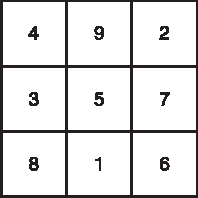
\includegraphics[scale=1.2]{2_lista_1_fig.pdf}
                        \caption{}
                        \label{fig:1}
                  \end{subfigure}
                  \hfil
                  \begin{subfigure}[c]{0.45\linewidth}
                        \centering
                        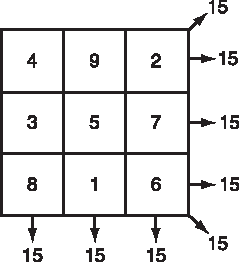
\includegraphics[scale=1.2]{2_lista_2_fig.pdf}
                        \caption{}
                        \label{fig:2}
                  \end{subfigure}
                  \hfil
                  \caption{Quadrado Mágico de Lo Shu.}
            \end{figure}

\end{enumerate}



\end{document}